\chapter{Methods}\label{sec:methods}

\section{System Model}\label{sec:system-model-1}

The system under study is a two-hop relay network with a single relay node. All methods in this chapter are described for the canonical setup of Chapter~\ref{sec:introduction}: SISO on both hops, i.i.d.\ Rayleigh fast fading, complex baseband, BPSK, uncoded BER.


\begin{figure}[H]
\centering
\resizebox{\textwidth}{!}{%
\begin{tikzpicture}[
  node distance=0.25cm and 0.2cm,
  box/.style={rectangle, draw, rounded corners=3pt, minimum width=1.7cm,
              minimum height=0.85cm, align=center, font=\small},
  arr/.style={->, thick, >=stealth}
]
\node[box] (src)   {Source\\tx bits};
\node[box, right=1.2cm of src]  (mod)   {BPSK\\Mod.};
\node[box, right=1.2cm of mod]  (ch1)   {Hop 1\\Channel};
\node[box, right=1.2cm of ch1]  (relay) {Relay\\$f_\theta$ / AF / DF};
\node[box, right=1.2cm of relay](ch2)   {Hop 2\\Channel};
\node[box, right=1.2cm of ch2](demod)   {demod};
\node[box, right=1.2cm of demod]  (dst)   {Dest.\\Rx bits};
\draw[arr] (src) -- (mod);
\draw[arr] (mod) -- (ch1);
\draw[arr] (ch1) -- node[above,font=\tiny]{Hop 1} (relay);
\draw[arr] (relay) -- (ch2);
\draw[arr] (ch2) -- node[above,font=\tiny]{Hop 2} (demod);
\draw[arr] (demod) -- (dst);
\end{tikzpicture}%
}
\caption{Two-hop relay system model: source transmits through two channels
         with a neural network relay in between.}
\label{fig:relay-system-simple}
\end{figure}


Source bits are BPSK-modulated, passed through Hop 1 (SISO Rayleigh), processed by the relay (classical or neural), transmitted over Hop 2 (SISO Rayleigh), and demodulated at the destination; no equalization is involved. Both hop channels are known perfectly at their respective receivers, per the conventions of Chapter~\ref{sec:introduction}.

\begin{equation}\protect\phantomsection\label{eq:two-hop-system}{\text{Source} \xrightarrow{\text{Hop 1}} \text{Relay} \xrightarrow{\text{Hop 2}} \text{Destination}
}\end{equation}
\addcontentsline{equ}{listequations}{\protect\numberline{\theequation}\quad two-hop-system}

\subsection{Modulation.}\label{sec:modulation}
The modulation throughout this thesis is BPSK, per the canonical setup: Binary Phase-Shift Keying maps a single bit to a real-valued symbol,

\begin{equation}\protect\phantomsection\label{eq:bpsk-mapping}{x = 1 - 2b, \quad b \in \{0, 1\} \implies x \in \{-1, +1\}}\end{equation}
\addcontentsline{equ}{listequations}{\protect\numberline{\theequation}\quad bpsk-mapping}

with hard-decision demodulation \(\hat{b} = \mathbb{1}[\hat{x} < 0]\) at the destination. The QPSK and 16-QAM extensions are defined in Section~\ref{sec:modulation-schemes} and evaluated in Chapter~\ref{sec:extensions}; further constellations are future work.




\subsection{Hop Model}\label{sec:hop-model}
Each hop applies a channel function followed by optional equalization (Equation~\ref{eq:hop-model-selection}):

\begin{equation}\protect\phantomsection\label{eq:hop-model-selection}{y = h(x, \text{SNR}) + n}
\end{equation}
\addcontentsline{equ}{listequations}{\protect\numberline{\theequation}\quad hop-model}


where \(h(\cdot)\) is the canonical Rayleigh fast-fading channel (the AWGN special case is retained for analytical calibration of the simulator).

\textbf{Power Normalization.} All relay strategies normalize their output power to ensure fair comparison:

\begin{equation}\protect\phantomsection\label{eq:power-normalization}{x_R \leftarrow x_R \cdot \sqrt{\frac{P_{\text{target}}}{P_{\text{current}}}}
}\end{equation}
\addcontentsline{equ}{listequations}{\protect\numberline{\theequation}\quad power-normalization}

\subsection{Relay Processing}\label{sec:relay-processing-methods}

On Hop 1 the relay's single receive antenna observes, as shown in Equation~\ref{eq:relay-received-siso}:

\begin{equation}\protect\phantomsection\label{eq:relay-received-siso}{y_R = x + n_1, \quad n_1 \sim \mathcal{N}(0, \sigma^2)
}\end{equation}
\addcontentsline{equ}{listequations}{\protect\numberline{\theequation}\quad relay-received-siso}

where the effective observation follows coherent compensation of the Rayleigh fading coefficient (Section~\ref{sec:system-model-1}). The relay applies its processing function to a sliding window of received samples and transmits a cleaner estimate \(\hat{x}_R = f_\theta(y_{R,i-w:i+w})\); classical AF/DF use \(w=0\). This is purely a noise-removal task: in the canonical SISO setup there is no inter-stream interference at any stage, and the destination demodulates the Hop-2 output directly with no equalizer.
\REV{Same modelling gap as in Section~1.1: Eq.~\ref{eq:relay-received-siso} states $n_1\sim\mathcal{N}(0,\sigma^2)$ with a \emph{fixed} variance, but after coherent compensation of $h\sim\mathcal{CN}(0,1)$ the per-symbol effective SNR is $|h|^2\gamma$ --- random, exponentially distributed --- not constant. The text says the right thing; the equation says the calibration case. Write the post-compensation observation as $\tilde y_R = |h_1|\,x + \tilde n_1$ (or condition on $|h|$) so the displayed math matches the canonical channel. Separately, in Eq.~\ref{eq:hop-model-selection} the symbol $h(\cdot)$ is used as the \emph{channel function} while $h$ elsewhere is the fading \emph{coefficient} --- rename one to avoid collision.}


\section{Relay Strategies}\label{sec:relay-strategies}

Nine relay strategies were implemented, spanning four learning paradigms. The selection of these nine strategies is designed to systematically explore the relay design space along three axes: 
\begin{enumerate}
    \item  the degree of processing (from no learning to deep generative models).
    \item the type of inductive bias (feedforward, recurrent, attention, generative).
    \item the model capacity (from 0 to 26K parameters). This section describes each strategy's architecture, training procedure, and the design rationale motivating each choice.
\end{enumerate}

\subsection{Selection and Classification of Relay Strategies
}

The selected nine relay strategies are drawn from four distinct architectural concepts:

\begin{enumerate*}[label=(\roman*), itemjoin={{, }}, itemjoin*={{, and }}, afterlabel=\ ]
\tightlist
\item classical methods (AF and DF)
\item supervised-learning models (MLP and hybrid MLP--DF)
\item generative models (VAE and CGAN)
\item sequential models (Transformers, Mamba-SSM, and Mamba-SSD)
\end{enumerate*}.

\begin{enumerate}
\item \textbf{Classical AF:} Gain amplification as shown in equation \ref{eq:af-gain}.  AF serves as the lower baseline. it performs no intelligent processing and simply rescales the received signal, preserving both signal and noise. Its end-to-end effective SNR is given in Equation~\ref{eq:af-snr}.
\item \textbf{Classical DF:} Demodulates, recovers bits and re-modulates clean BPSK symbols. DF serves as the upper classical baseline: it performs the maximum possible classical processing (full signal regeneration). At high SNR, DF approaches error-free relay operation. Its theoretical BER follows the error-composition formula of Equation~\ref{eq:df-ber-hops}.

\item \textbf{Supervised MLP (Minimal):} A two-layer feedforward neural network (multi-layer perceptron, MLP) with 169 parameters following the relay architecture defined in Equation~\ref{eq:mlp-relay},

where \(\mathbf{w} \in \mathbb{R}^5\) is a sliding window of received symbols (\(w=2\) neighbors on each side), and the hidden layer has 24 neurons. Parameters: \((5 \times 24 + 24) + (24 \times 1 + 1) = 169\).

\begin{quote}
\textbf{Architecture note:} The MLP relay is a standard discriminative dual-layer perceptron trained with supervised learning (MSE loss on input--output pairs). In contrast, the generative models in this study are the VAE (§6.3, Generative Models) and CGAN, which learn to \emph{sample from} or \emph{approximate} the data distribution. The MLP relay simply learns a deterministic mapping \(f: \mathbb{R}^5 \to [-1,+1]\) from a noisy observation window to a denoised symbol estimate : a classical regression task.
\end{quote}

\emph{Design rationale:} The tanh output activation naturally constrains the output to \([-1, +1]\), matching the BPSK symbol range. The ReLU hidden layer provides the non-linearity needed to approximate the Bayes-optimal soft threshold \(\tanh(y/\sigma^2)\). With 24 hidden neurons and a 5-dimensional input, the network has approximately 34 parameters per input dimension : sufficient for the low-complexity denoising task while avoiding overfitting. He initialization is used for ReLU layers to maintain proper gradient flow.
\REV{Resolved (activation): checked against the implementation --- \texttt{MinimalGenAIRelay} (\texttt{relaynet/relays/genai.py}) uses a \emph{ReLU} hidden layer (\texttt{np.maximum(0, z1)}) and a \emph{tanh} output, exactly as stated here and in Eq.~\ref{eq:mlp-relay}. So Methods is correct; the imprecise text was the experiment-configuration lines in Chapters~\ref{sec:experiments}--\ref{sec:extensions} that list ``NN activation: tanh'' without qualification --- those refer to the \emph{output} activation and have been reworded to ``ReLU hidden, tanh output.'' (Parameter count $(5{\times}24+24)+(24{\times}1+1)=169$ confirmed.)}

Training uses MSE loss with multi-SNR training data (i.e. )  5, 10 and 15 dB), 25,000 samples, and 100 epochs with a learning rate of 0.01.

\item \textbf{Hybrid:} SNR-adaptive relay that switches between MLP (low SNR) and DF (high SNR) based on a learned threshold. Combines the AI advantage at low SNR with the zero-error classical approach at high SNR. Same 169 parameters as MLP.

  \emph{Design rationale:} The Hybrid relay is motivated by the observation (confirmed empirically) that AI relays outperform DF only at low SNR, while DF is optimal at high SNR. By introducing a switching threshold, the Hybrid relay automatically selects the better strategy for each operating condition. The threshold is determined empirically from the training data by finding the SNR at which MLP and DF BER curves cross. This approach requires no additional parameters beyond those of the MLP sub-network.

  Training points at the relay node: SNR = \textbf{5, 10, 15 dB} (same trained MLP sub-network as the Minimal MLP relay).

\item \textbf{Generative VAE:} Probabilistic relay with encoder \(q_\phi(\mathbf{z}|\mathbf{x})\) mapping to a latent space and decoder \(p_\theta(\mathbf{x}|\mathbf{z})\) reconstructing the signal. Architecture: encoder \((7 \to 32 \to 16 \to \mu, \sigma^2(8))\), decoder \((8 \to 16 \to 32 \to 1)\). Total: 1,777 parameters. Trained with \(\beta\)-VAE loss (\(\beta=0.1\)) for 100 epochs.

  Training points at the relay node: SNR = \textbf{5, 10, 15 dB}.

  \emph{Design rationale:} The low \(\beta = 0.1\) prioritizes reconstruction quality over latent space regularization, appropriate for a task where accurate signal recovery is paramount. The 8-dimensional latent space provides sufficient representational capacity for the BPSK signal manifold while maintaining a tractable KL divergence. The encoder window of 7 symbols provides local context.
\item  \textbf{Generative CGAN (WGAN-GP):} Adversarial relay with a generator conditioned on the noisy signal and a critic providing the training signal. Generator: \((7+8 \to 32 \to 32 \to 16 \to 1)\), Critic: \((1+7 \to 32 \to 16 \to 1)\). Total: 2,946 parameters. Trained with Wasserstein loss, gradient penalty (\(\lambda=10\)), and L1 reconstruction loss (\(\lambda_{\text{L1}}=100\)) for 200 epochs.

  Training points at the relay node: SNR = \textbf{5, 10, 15 dB}.

  \emph{Design rationale:} The high \(\lambda_{\text{L1}} = 100\) ensures that the generator is primarily supervised by the reconstruction loss, with the adversarial term acting as a regularizer that encourages outputs to lie on the clean signal manifold. The noise vector \(\mathbf{z} \in \mathbb{R}^8\) provides the stochastic input needed by the GAN framework. The 5:1 critic-to-generator update ratio follows the WGAN-GP recommendation for stable critic training. The doubled epoch count (200 vs.~100) compensates for the slower per-step convergence of adversarial training.

\item  \textbf{Sequential models: Transformer:} Multi-head self-attention over a window of 11 symbols. Architecture: \(d_{\text{model}}=32\), 4 attention heads, 2 encoder layers, feedforward dimension 128. Total: 17,697 parameters. Trained for 100 epochs with Adam optimizer (\(\text{lr}=10^{-3}\)).

  Training points at the relay node: SNR = \textbf{5, 10, 15 dB}.

  \emph{Design rationale:} The Transformer is included as the dominant sequence architecture in modern deep learning. The 11-symbol window provides the same temporal context as the S6/SSD models. With \(d_{\text{model}} = 32\) and 4 heads, each head operates in an 8-dimensional subspace, which is sufficient for capturing the local noise structure. The feedforward dimension of 128 (\(4 \times d_{\text{model}}\)) follows the standard Transformer expansion ratio.
\item  \textbf{Sequential models: Mamba S6} Selective state space model with input-dependent state transitions. Architecture: \(d_{\text{model}}=32\), \(d_{\text{state}}=16\), 2 Mamba blocks with residual connections. Total: 24,001 parameters. Each block applies: LayerNorm → expand (\(32 \to 64\)) → split to Conv1D/SiLU/S6 main branch and SiLU gate → contract (\(64 \to 32\)) → residual. Trained for 100 epochs with Adam optimizer (\(\text{lr}=10^{-3}\)).

  Training points at the relay node: SNR = \textbf{5, 10, 15 dB}.

  \emph{Design rationale:} The expand factor of 2 (\(32 \to 64\)) doubles the internal dimension during the S6 scan, providing richer state dynamics. The state dimension \(N = 16\) means each S6 layer implements a 16th-order adaptive filter : substantially more expressive than classical Wiener or matched filters. LayerNorm and residual connections prevent gradient degradation across layers. The SiLU gating provides multiplicative interactions that help the model learn sharp decision boundaries.

\item \textbf{Sequential models: Mamba2 (SSD)} Structured State Space Duality model that replaces the sequential S6 recurrence with a chunk-parallel structured matrix multiply. Architecture: \(d_{\text{model}}=32\), \(d_{\text{state}}=16\), chunk size 8, 2 Mamba-2 blocks with SiLU gating and residual connections. Total: 26,179 parameters. Each block applies: LayerNorm → parallel gate/SSD branches → SiLU gate → contract (\(64 \to 32\)) → residual. The SSD layer builds a lower-triangular causal kernel \(M\) per chunk and applies it via batched matmul, with inter-chunk state passing for continuity. Trained for 100 epochs with Adam optimizer (\(\text{lr}=10^{-3}\)) and gradient clipping (\(\|\nabla\| \le 1\)).

  Training points at the relay node: SNR = \textbf{5, 10, 15 dB}.

  \emph{Design rationale:} The chunk size of 8 is chosen to balance parallelism (larger chunks = fewer sequential inter-chunk passes) against memory cost (the \(L \times L\) SSM matrix scales quadratically with chunk size). At the 11-symbol window, this yields 2 chunks (8 + 3), with a single inter-chunk state pass. Gradient clipping at norm 1.0 prevents the exponential blowup of gradients through the cumulative matrix products in the SSD computation. The S4D-style initialization \(A_{\text{log}} = \log(1, 2, \dots, N)\) provides geometrically spaced decay rates, enabling the model to simultaneously capture short-range and medium-range dependencies.

\end{enumerate}

\section{Simulation Framework}\label{sec:simulation-framework}

\subsection{Monte Carlo BER Estimation}\label{sec:monte-carlo-ber-estimation}

BER is estimated through Monte Carlo simulation, which provides an unbiased estimate of the true BER at each SNR point. The simulation parameters are:

\begin{itemize}
\tightlist
\item
  \textbf{Bits per trial:} 10,000
\item
  \textbf{Trials per SNR:} 10 (independent random seeds)
\item
  \textbf{Total bits per SNR point:} 100,000
\item
  \textbf{SNR range:} 0 to 20 dB (step: 2 dB), yielding 11 evaluation points
\item
  \textbf{Random seed control:} Each trial uses a unique seed for bit generation and noise realization
\end{itemize}

\textbf{BER Computation:}

\begin{equation}\protect\phantomsection\label{eq:ber-estimate}{\hat{P}_e = \frac{1}{N}\sum_{i=1}^{N} \mathbb{\textbf{1}}(b_i \neq \hat{b}_i)
}\end{equation}
\addcontentsline{equ}{listequations}{\protect\numberline{\theequation}\quad ber-estimate}

where \(\mathbb{\text{1}}(\cdot)\) is the indicator function and \(N = 10{,}000\) is the number of bits per trial. By the central limit theorem, for large \(N\) and moderate BER (say \(P_e \geq 10^{-3}\)), the per-trial BER estimate is approximately normally distributed with variance \(P_e(1-P_e)/N\).

\textbf{Confidence Intervals.} The 95\% confidence interval is computed from the \(M = 10\) independent trial estimates as:

\begin{equation}\protect\phantomsection\label{eq:confidence-interval}{\text{CI}_{95\%} = \bar{P}_e \pm t_{0.025, M-1} \cdot \frac{s}{\sqrt{M}}
}\end{equation}
\addcontentsline{equ}{listequations}{\protect\numberline{\theequation}\quad confidence-interval}

where \(\bar{P}_e\) is the sample mean BER across trials, \(s\) is the sample standard deviation, and \(t_{0.025, 9} = 2.262\) is the critical value of the Student's \(t\)-distribution with 9 degrees of freedom. At low BER (\(\hat{P}_e \lesssim 10^{-4}\)), the normal approximation may become unreliable due to the small number of observed errors; however, in this regime the relay methods converge and the relative ranking is stable.

\textbf{BER resolution.} With \(N \cdot M = 100{,}000\) total bits per SNR point, the minimum detectable BER is approximately \(1/N = 10^{-4}\) per trial, or \(10^{-5}\) for the aggregate. BER values below this threshold are reported as 0.

\textbf{Per-experiment simulation budgets.} The budget above ($M=10$ trials $\times\,N=10{,}000$ bits $=100{,}000$ bits per SNR point) applies to the canonical relay comparison and the parameter-normalization/complexity study (E2--E3). Two experiments use different budgets, stated in their respective sections: the channel-model validation (E1, Section~\ref{sec:channel-model-validation-simulative}) uses $20\times50{,}000 = 1{,}000{,}000$ bits per SNR point for tight validation intervals, and the unknown-channel study (Chapter~\ref{sec:unknown-channels}) uses $5\times50{,}000 = 250{,}000$ bits per SNR point. Because the Wilcoxon signed-rank test at $M=5$ cannot attain $p<0.05$ (its smallest two-sided $p$ is $2^{-4}=0.0625$), formal significance testing is reported only for the $M=10$ experiments; the unknown-channel results are reported with means and 95\% confidence intervals rather than Wilcoxon $p$-values.

\REV{Fix applied (review finding \#3): the per-experiment budget paragraph above replaces the former blanket claim (E1 $20\times50$k, E2--E3 $10\times10$k, Ch7 $5\times50$k), and the $M=5$ Wilcoxon caveat is now stated explicitly. The abstract has been reworded to match.}

\subsection{Statistical Significance Testing}\label{sec:statistical-significance-testing}

Differences between relay methods are assessed using the \textbf{Wilcoxon signed-rank test}, a non-parametric paired test. For each pair of relay strategies \((A, B)\) at each SNR point, the test compares the \(M = 10\) paired BER observations (Equation~\ref{eq:wilcoxon-test}):

\begin{equation}\protect\phantomsection\label{eq:wilcoxon-test}{H_0: \text{median}(P_{e,A} - P_{e,B}) = 0 \quad \text{vs.} \quad H_1: \text{median}(P_{e,A} - P_{e,B}) \neq 0
}\end{equation}
\addcontentsline{equ}{listequations}{\protect\numberline{\theequation}\quad wilcoxon-test}

The Wilcoxon test is preferred over the parametric paired \(t\)-test for two reasons: (i) BER distributions are bounded (\([0, 0.5]\)) and potentially skewed, violating the normality assumption, and (ii) the test is robust to outlier trials. The significance level is set at \(\alpha = 0.05\).

\subsection{Training Protocol}\label{sec:training-protocol}

All AI relays are trained \textbf{once} at the beginning of each experiment using: - \textbf{Multi-SNR training data:} Signals generated at SNR = 5, 10, 15 dB in equal proportions - \textbf{Training samples:} 25,000 (supervised), 20,000 (generative), 10,000 (sequence models) - \textbf{Single training per channel:} The same trained model is evaluated across all SNR points

The multi-SNR training protocol is critical: training at a single SNR would produce a model that performs well at that SNR but poorly at others (overfitting to a specific noise level). By training at three representative SNR values spanning the low-to-moderate range, the network learns a robust denoising function that generalizes across operating conditions. The SNR values 5, 10, 15 dB were chosen to cover the regime where AI relays provide the most benefit (low-to-medium SNR).

\textbf{Impact of sparse SNR training grid.} Because models are trained at only three SNR points (\(\{5,10,15\}\) dB) but evaluated over eleven points (\(0\) to \(20\) dB, step \(2\)), performance reflects two regimes: (i) \textbf{interpolation} within the trained span (approximately \(4\)--\(16\) dB), where BER is generally stable, and (ii) \textbf{extrapolation} at the edges (\(0\)--\(2\) dB and \(18\)--\(20\) dB), where mild degradation may occur due to noise-statistics mismatch. In the present results, this sparse-grid effect is secondary: the relay ranking remains consistent across the full evaluated SNR range.

\textbf{Training method (what is trained, where it is trained).} Training is performed \textbf{offline} before BER sweeps. Only the seven AI relays are optimized (MLP, Hybrid's MLP sub-network, VAE, CGAN, Transformer, Mamba S6, Mamba-2 SSD); AF and DF are analytical baselines and have no trainable parameters. Training data are synthetically generated source/channel pairs under the multi-SNR protocol, with model-specific losses (MSE for supervised relays, ELBO for VAE, WGAN-GP + L1 for CGAN, Adam-based supervised loss for sequence models). Compute placement follows implementation: NumPy models (MLP/Hybrid) train on CPU, while PyTorch models train on CPU or CUDA depending on device availability/configuration. After training, weights are checkpointed and reused across all SNR evaluations; BER curves are then produced in \textbf{inference-only} mode without further parameter updates.

\textbf{Weight initialization.} He initialization \cite{He2015DelvingRectifiers} is used for all layers with ReLU activation (\(W \sim \mathcal{N}(0, 2/n_{\text{in}})\)), while Xavier initialization is used for layers with tanh activation (\(W \sim \mathcal{N}(0, 1/n_{\text{in}})\)). These initialization schemes maintain proper gradient magnitude through the network layers, preventing both vanishing and exploding gradients during training.

\textbf{Optimizer settings.} All PyTorch-based models use the Adam optimizer with \(\beta_1 = 0.9\), \(\beta_2 = 0.999\), \(\epsilon = 10^{-8}\) (defaults). The MLP and Hybrid relays use a simple SGD implementation in NumPy with constant learning rate \(\eta = 0.01\).

\subsection{Reproducibility and Weight Management}\label{sec:reproducibility-and-weight-management}

All experiments use controlled random seeds at both the source (bit generation) and noise (per-trial seeding) levels to ensure reproducible results. Specifically, for seed \(s\) and trial \(t\), the random state is initialized as \(\text{seed}(s \cdot 1000 + t)\), ensuring that each trial is independent while the overall experiment is deterministic.

A \textbf{weight checkpoint system} saves trained model parameters to disk after training completes, enabling experiment resumption without retraining. This is particularly important for the CGAN (2-hour training time) and sequence models (24--37 minutes). The checkpoint system supports: - Automatic save after training with architecture metadata - Resume from saved weights with architecture validation - Seed-specific weight directories (e.g., \texttt{trained\_weights/seed\_42/})

The framework includes 126 automated tests (pytest) covering all modules: channels, modulation, relay strategies, simulation, statistics, and weight management, with 100\% pass rate.

\section{Normalized Parameter Comparison}\label{sec:normalized-parameter-comparison}

A fundamental confound in comparing AI architectures is that different models have vastly different parameter counts: from 169 (MLP) to 26,179 (Mamba-2 SSD) : a ratio of 155:1. Performance differences between these models could reflect either (a) the superiority of one architecture's inductive bias, or (b) the simple advantage of having more learnable parameters. To disentangle these two effects, all seven AI models were scaled to approximately 3,000 parameters, providing a controlled comparison where model capacity is held constant.

\textbf{Choice of target parameter count.} The target of \textasciitilde3,000 parameters was chosen as a compromise: it is large enough that all architectures can express a reasonable denoising function (avoiding underfitting), yet small enough that the normalization represents a meaningful reduction for the larger models (Transformer: 5.9× reduction, Mamba S6: 7.9×, Mamba-2: 8.7×). The MLP model is scaled \textbf{up} from 169 to 3,004 parameters, testing whether additional capacity benefits the simple feedforward architecture.

\textbf{Scaling methodology.} Each architecture's hyperparameters were adjusted to reach the target while preserving its essential structure:

\begin{longtable}[]{@{}
  >{\raggedright\arraybackslash}p{(\linewidth - 4\tabcolsep) * \real{0.3333}}
  >{\raggedright\arraybackslash}p{(\linewidth - 4\tabcolsep) * \real{0.3333}}
  >{\raggedright\arraybackslash}p{(\linewidth - 4\tabcolsep) * \real{0.3333}}@{}}
\caption{Normalized 3K-parameter model configurations: parameter count and scaling method for each architecture.}\label{tbl:table28}\tabularnewline
\toprule\noalign{}
\begin{minipage}[b]{\linewidth}\raggedright
Model
\end{minipage} & \begin{minipage}[b]{\linewidth}\raggedright
Parameters
\end{minipage} & \begin{minipage}[b]{\linewidth}\raggedright
Scaling Method
\end{minipage} \\
\midrule\noalign{}
\endfirsthead
\toprule\noalign{}
\begin{minipage}[b]{\linewidth}\raggedright
Model
\end{minipage} & \begin{minipage}[b]{\linewidth}\raggedright
Parameters
\end{minipage} & \begin{minipage}[b]{\linewidth}\raggedright
Scaling Method
\end{minipage} \\
\midrule\noalign{}
\endhead
\bottomrule\noalign{}
\endlastfoot
MLP-3K & 3,004 & Increased window (5→11) and hidden (24→231) \\
Hybrid-3K & 3,004 & Same as MLP-3K + DF switching \\
VAE-3K & 3,037 & Increased window (7→11), adjusted latent/hidden \\
CGAN-3K & 3,004 & Increased window (7→11), adjusted hidden layers \\
Transformer-3K & 3,007 & Reduced d\_model (32→18), heads (4→2), layers (2→1) \\
Mamba-3K & 3,027 & Reduced d\_model (32→16), d\_state (16→6), layers (2→1) \\
Mamba2-3K & 3,004 & Reduced d\_model (32→15), d\_state (16→6), layers (2→1) \\
\end{longtable}

\textbf{Parameter counting convention.} All learnable parameters are counted, including biases, normalization parameters (LayerNorm gain/bias), and projection matrices. Non-learnable buffers (e.g., positional encoding tables, fixed \(\mathbf{A}\) matrices) are excluded. The counts are verified programmatically via \texttt{sum(p.numel()\ for\ p\ in\ model.parameters()\ if\ p.requires\_grad)}.

\textbf{Unified input window.} All 3K models use a window size of 11 (vs.~5 for original MLP/Hybrid, and 7 for original VAE/CGAN), providing a common input context. This ensures that differences in performance reflect architectural inductive biases rather than differences in the amount of input information available.

This normalization isolates the effect of architectural choice from the confound of parameter count, providing insights into which inductive biases are most beneficial for the relay denoising task. If performance converges at equal parameter budgets, the conclusion is that parameter count : not architecture : is the dominant factor. If significant gaps persist, the conclusion is that architectural inductive biases provide meaningful advantages beyond raw capacity.

\section{Extension Methods: QPSK and 16-QAM}\label{sec:modulation-schemes}

The core experiments use BPSK exclusively, per the canonical setup. To test whether the canonical findings generalize to complex constellations, the extension study of Chapter~\ref{sec:extensions} evaluates QPSK and 16-QAM. This section defines the two constellations, the I/Q-splitting technique that lets real-valued relays process complex signals, and the joint 2D classification formulation that removes I/Q splitting's structural limitation.

\subsection{QPSK : Gray-Coded Quadrature Phase-Shift Keying}\label{sec:qpsk-gray-coded-quadrature-phase-shift-keying}

Quadrature Phase-Shift Keying maps pairs of bits \((b_0, b_1)\) to complex symbols \cite{ProakisSalehi2008DigitalComm}:

\begin{equation}\protect\phantomsection\label{eq:qpsk-mapping}{x = \frac{(1 - 2b_0) + j(1 - 2b_1)}{\sqrt{2}}
}\end{equation}
\addcontentsline{equ}{listequations}{\protect\numberline{\theequation}\quad qpsk-mapping}

yielding four constellation points at \(\{(\pm 1 \pm j)/\sqrt{2}\}\) with unit average power (\(E_s = 1\)). The Gray coding ensures that adjacent constellation points differ by exactly one bit:

\begin{longtable}[]{@{}lll@{}}
\caption{QPSK Gray-coded symbol mapping: bit pairs to complex symbols.}\label{tbl:table29}\tabularnewline
\toprule\noalign{}
Bit pair \((b_0, b_1)\) & Symbol & Quadrant \\
\midrule\noalign{}
\endfirsthead
\toprule\noalign{}
Bit pair \((b_0, b_1)\) & Symbol & Quadrant \\
\midrule\noalign{}
\endhead
\bottomrule\noalign{}
\endlastfoot
00 & \((+1+j)/\sqrt{2}\) & I \\
01 & \((+1-j)/\sqrt{2}\) & IV \\
11 & \((-1-j)/\sqrt{2}\) & III \\
10 & \((-1+j)/\sqrt{2}\) & II \\
\end{longtable}

Demodulation applies independent sign decisions on each component: \(\hat{b}_0 = \mathbb{1}(\text{Re}(\hat{x}) < 0)\) and \(\hat{b}_1 = \mathbb{1}(\text{Im}(\hat{x}) < 0)\). The spectral efficiency is 2 bits/symbol, double that of BPSK.

\textbf{Theoretical QPSK BER.} For uncoded QPSK over an AWGN channel, the BER per bit equals the BPSK BER at the same \(E_b/N_0\) because each I/Q component carries an independent BPSK stream \cite{ProakisSalehi2008DigitalComm}:

\begin{equation}\protect\phantomsection\label{eq:qpsk-ber}{P_b^{\text{QPSK}} = Q\!\left(\sqrt{\frac{2E_b}{N_0}}\right) = P_b^{\text{BPSK}}
}\end{equation}
\addcontentsline{equ}{listequations}{\protect\numberline{\theequation}\quad qpsk-ber}

The advantage of QPSK is doubled throughput for the same BER and per-bit energy.

\subsection{16-QAM : Gray-Coded Quadrature Amplitude Modulation}\label{sec:qam-gray-coded-quadrature-amplitude-modulation}

16-QAM maps groups of four bits \((b_0, b_1, b_2, b_3)\) to one of 16 complex constellation points arranged on a \(4 \times 4\) rectangular grid (Figure~\ref{fig:fig8}c). Each axis (I and Q) uses independent Gray-coded PAM-4 mapping \cite{ProakisSalehi2008DigitalComm}:

\begin{equation}\protect\phantomsection\label{eq:qam16-mapping}{I = \frac{L(b_0, b_1)}{\sqrt{10}}, \quad Q = \frac{L(b_2, b_3)}{\sqrt{10}}, \quad x = I + jQ
}\end{equation}
\addcontentsline{equ}{listequations}{\protect\numberline{\theequation}\quad qam16-mapping}

where \(L(\cdot)\) maps bit pairs to PAM-4 levels using Gray coding:

\begin{longtable}[]{@{}llll@{}}
\caption{16-QAM PAM-4 Gray-coded level mapping for in-phase and quadrature components.}\label{tbl:table30}\tabularnewline
\toprule\noalign{}
Bit pair & Level & Bit pair & Level \\
\midrule\noalign{}
\endfirsthead
\toprule\noalign{}
Bit pair & Level & Bit pair & Level \\
\midrule\noalign{}
\endhead
\bottomrule\noalign{}
\endlastfoot
00 & \(+3\) & 11 & \(-1\) \\
01 & \(+1\) & 10 & \(-3\) \\
\end{longtable}

The normalization factor \(\sqrt{10}\) ensures unit average symbol power: \(E[|x|^2] = \frac{2 \cdot (9+1+1+9)}{4 \cdot 10} = 1\). Adjacent constellation points differ by one bit (Gray property), minimizing the BER for a given symbol error rate.

Demodulation quantises each received component to the nearest PAM-4 level using decision boundaries at \(\{-2, 0, +2\}/\sqrt{10}\) and maps back to bits via the inverse Gray table. The spectral efficiency is 4 bits/symbol.

\textbf{Theoretical 16-QAM BER.} The approximate BER for 16-QAM over AWGN is: (Equation~\ref{eq:qam16-ber})

\begin{equation}\protect\phantomsection\label{eq:qam16-ber}{P_b^{\text{16-QAM}} \approx \frac{3}{8} \operatorname{erfc}\!\left(\sqrt{\frac{2E_b}{5N_0}}\right)
}\end{equation}
\addcontentsline{equ}{listequations}{\protect\numberline{\theequation}\quad qam16-ber}

At the same \(E_b/N_0\), 16-QAM has a higher BER than BPSK or QPSK due to the reduced Euclidean distance between constellation points. The trade-off is 4× throughput improvement.

\subsection{Constellation Diagram Summary}\label{sec:constellation-diagram-summary}

Figure~\ref{fig:fig8} presents the constellation diagrams for the modulation schemes appearing in this thesis. The progression from BPSK (2 points on the real axis) through QPSK (4 points on the unit circle) to 16-QAM (16 points on a rectangular grid) illustrates the fundamental trade-off between spectral efficiency and noise robustness: higher-order constellations pack more bits per symbol but reduce the minimum Euclidean distance between points, increasing the BER at a given SNR.

\begin{figure}[H]
\centering
\pandocbounded{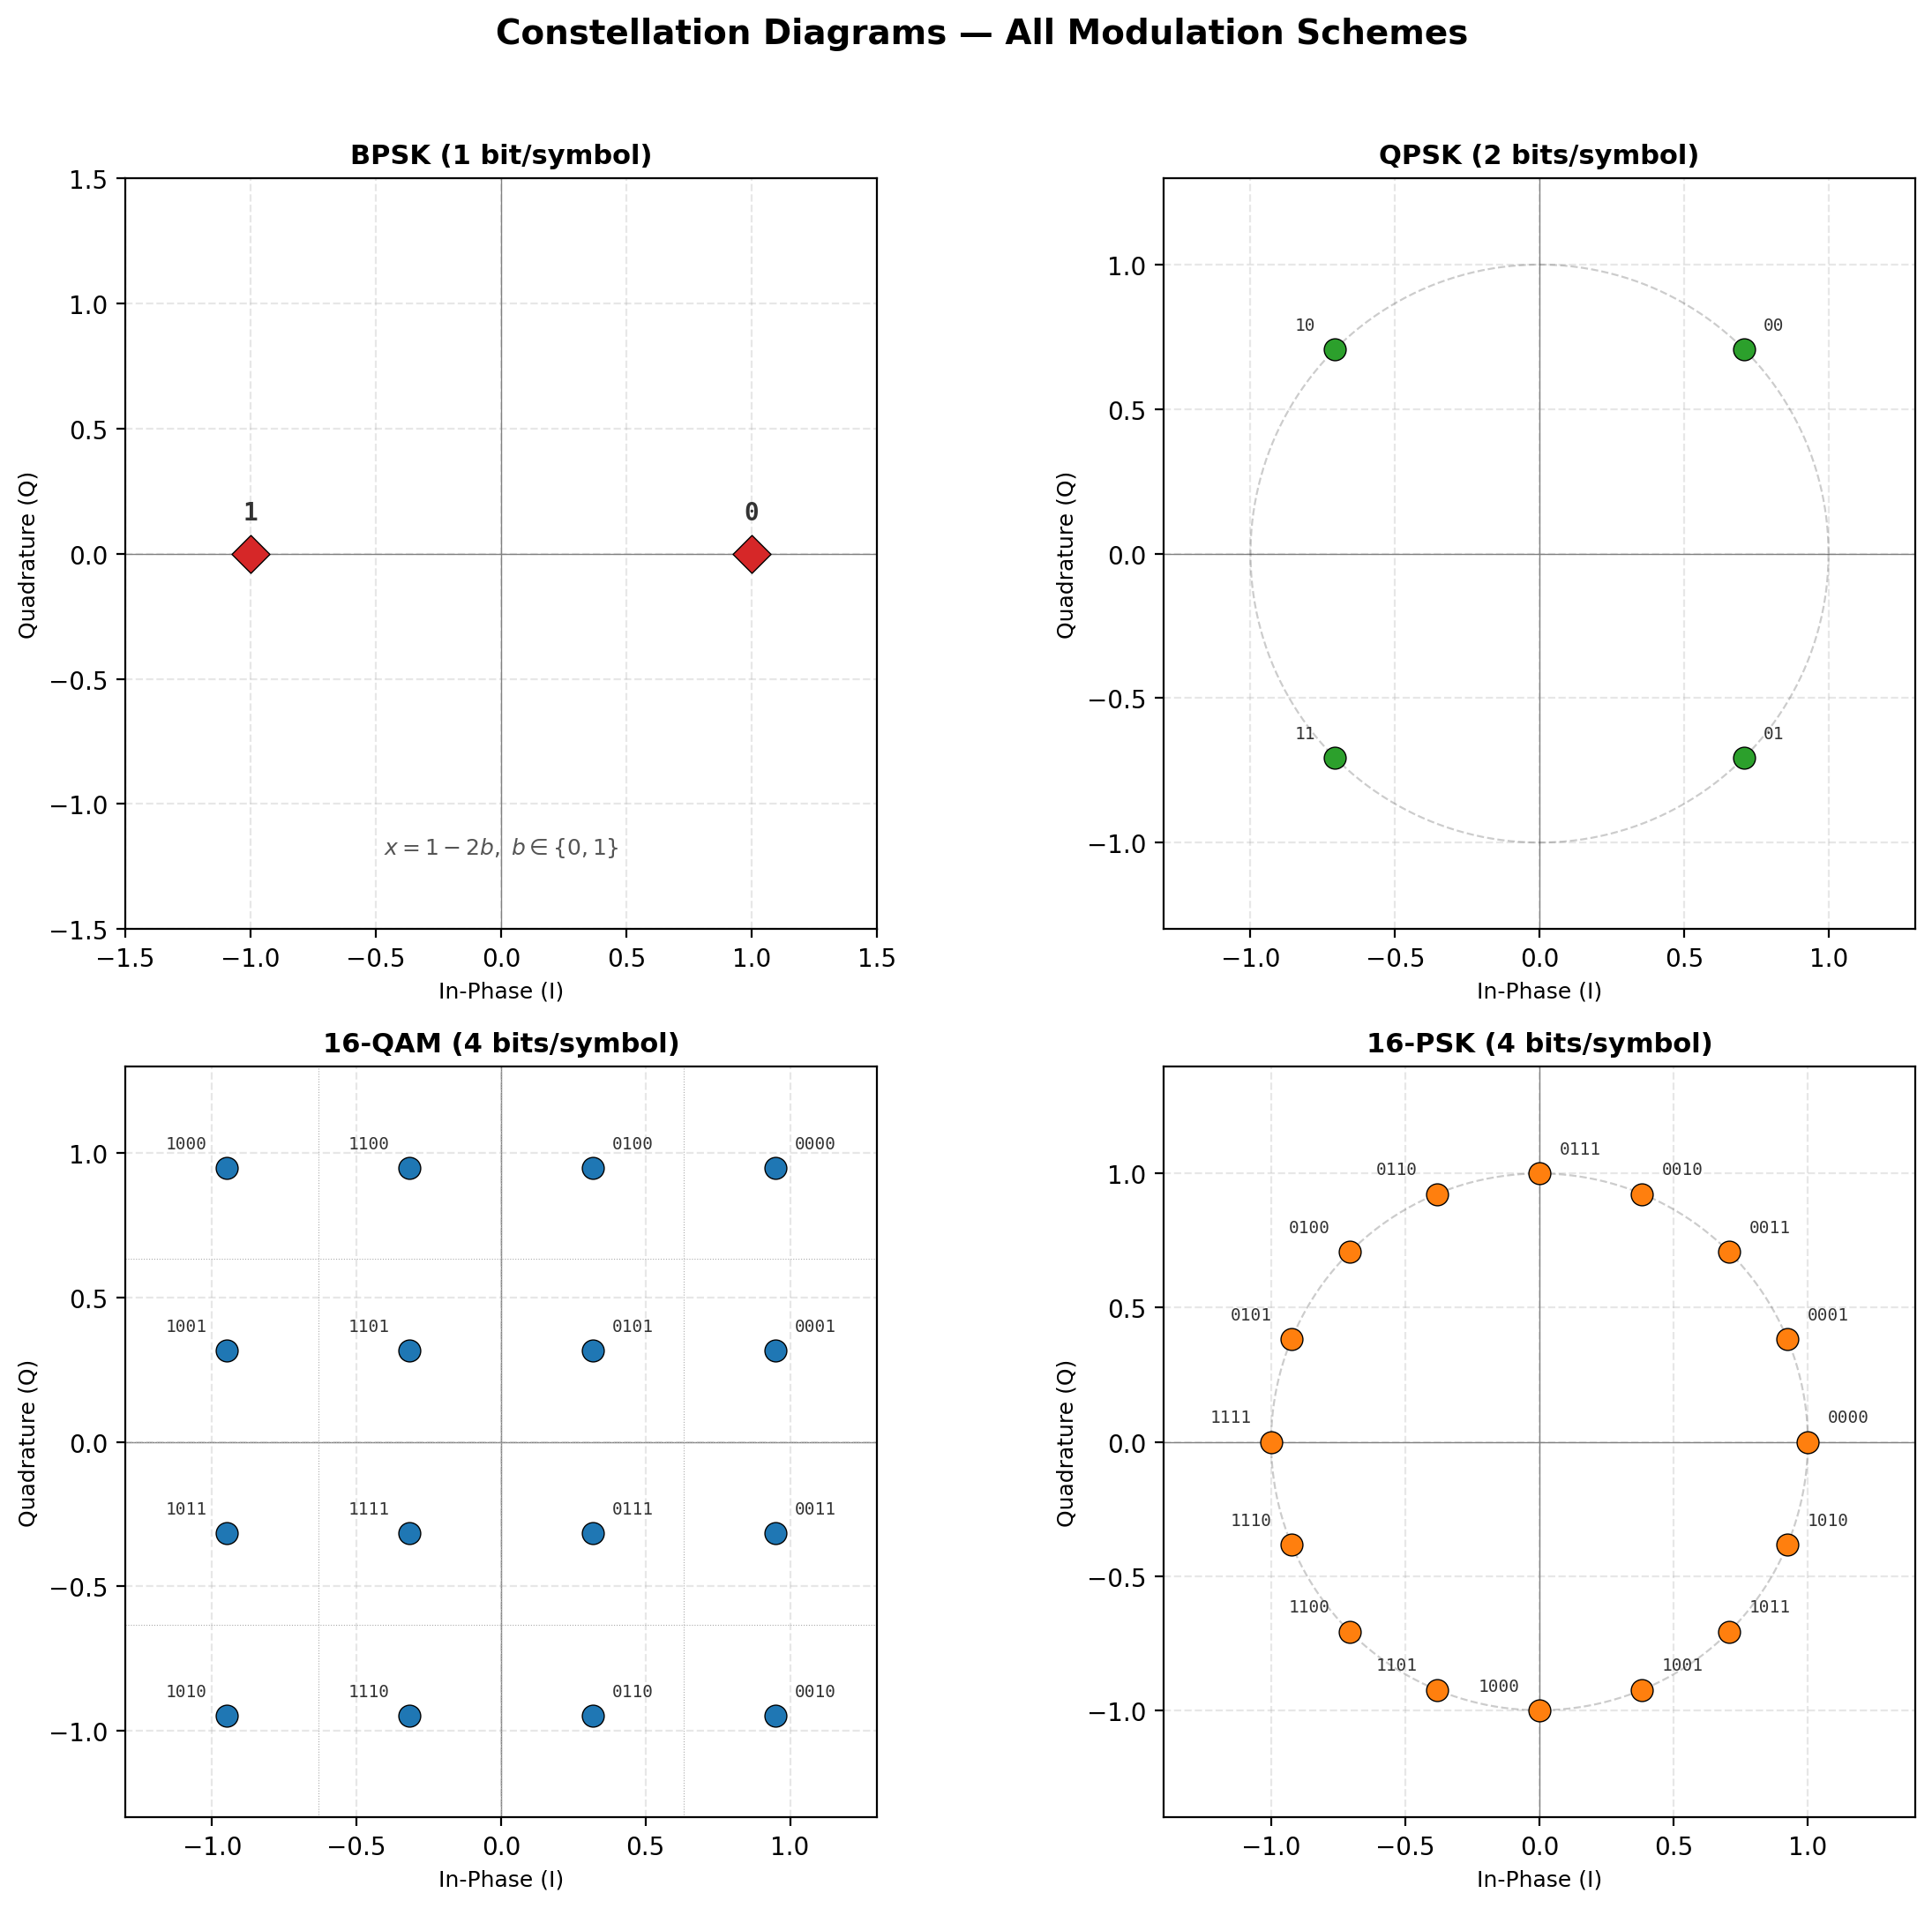
\includegraphics[width=\linewidth,height=0.45\textheight,keepaspectratio]{results/modulation/constellation_diagrams.png}}
\caption{Constellation diagrams. (a) BPSK: 2 real-valued symbols at \(\pm 1\). (b) QPSK: 4 Gray-coded symbols on the unit circle. (c) 16-QAM: 16 Gray-coded symbols on a \(4 \times 4\) rectangular grid with decision boundaries (dotted lines). (d) 16-PSK, shown for completeness only; it is not studied in this work. All constellations are normalised to unit average power.}\label{fig:fig8}
\end{figure}

\subsection{I/Q Splitting for AI Relay Processing of Complex Constellations}\label{sec:iq-splitting-for-ai-relay-processing-of-complex-constellations}


\begin{equation}\protect\phantomsection\label{eq:iq-splitting}{\hat{x}_R = f_\theta(\text{Re}(y_R)) + j \cdot f_\theta(\text{Im}(y_R))
}\end{equation}
\addcontentsline{equ}{listequations}{\protect\numberline{\theequation}\quad iq-splitting}

\textbf{Justification and caveat.} For rectangular constellations (QPSK, QAM), the I and Q components carry independent information and are corrupted by independent noise, so per-axis denoising with a shared real-valued function is a natural and parameter-efficient decomposition. It is, however, a \emph{restriction} of the hypothesis class to axis-separable functions, not an equivalence to joint 2D processing: per-axis errors accumulate independently, which is precisely the structural limitation quantified and then removed by the joint 2D classification formulation of Section~\ref{sec:d-joint-classification-as-an-alternative-to-iq-splitting}.

\textbf{Relay-specific handling:}

\begin{longtable}[]{@{}
  >{\raggedright\arraybackslash}p{(\linewidth - 4\tabcolsep) * \real{0.3333}}
  >{\raggedright\arraybackslash}p{(\linewidth - 4\tabcolsep) * \real{0.3333}}
  >{\raggedright\arraybackslash}p{(\linewidth - 4\tabcolsep) * \real{0.3333}}@{}}
\caption{Relay-specific complex signal handling strategies and rationale.}\label{tbl:table31}\tabularnewline
\toprule\noalign{}
\begin{minipage}[b]{\linewidth}\raggedright
Relay type
\end{minipage} & \begin{minipage}[b]{\linewidth}\raggedright
Complex signal processing
\end{minipage} & \begin{minipage}[b]{\linewidth}\raggedright
Rationale
\end{minipage} \\
\midrule\noalign{}
\endfirsthead
\toprule\noalign{}
\begin{minipage}[b]{\linewidth}\raggedright
Relay type
\end{minipage} & \begin{minipage}[b]{\linewidth}\raggedright
Complex signal processing
\end{minipage} & \begin{minipage}[b]{\linewidth}\raggedright
Rationale
\end{minipage} \\
\midrule\noalign{}
\endhead
\bottomrule\noalign{}
\endlastfoot
\textbf{AF} & Amplifies complex signal directly & Power normalization (\(\|y\|^2\)) is valid for complex vectors \\
\textbf{AI relays} & I/Q splitting (process Re and Im separately) & Real-valued networks; independence of I/Q in rectangular constellations \\
\end{longtable}

\textbf{Limitation for 16-QAM with AI relays.} For 16-QAM, each I/Q component takes four amplitude levels (\(\{-3, -1, +1, +3\}/\sqrt{10}\)) rather than the binary \(\{\pm 1\}\) of BPSK. The BPSK-trained relays, which use \(\tanh\) activations bounded in \([-1, +1]\), may not faithfully reproduce the multi-level structure. This provides a natural test of generalisation: if AI relays degrade significantly on 16-QAM but not on QPSK, it indicates that the BPSK training generalises to binary-per-component signals (QPSK) but not to multi-level signals (16-QAM). Such a finding would motivate modulation-specific relay training.


\subsection{2D Joint Classification as an Alternative to I/Q Splitting}\label{sec:d-joint-classification-as-an-alternative-to-iq-splitting}

The I/Q splitting approach (Section 3.7.6) treats each axis of the complex constellation independently, classifying each component into \(\sqrt{M}\) amplitude levels. For 16-QAM this yields two independent 4-class problems. While valid under the assumption of I/Q independence, this formulation introduces a \textbf{structural limitation}: (Equation~\ref{eq:joint-classification}) classification errors on the I and Q axes accumulate independently, producing a BER floor that cannot be reduced regardless of model capacity.

An alternative formulation treats the relay as a \textbf{joint 2D classifier} over all \(M\) constellation points simultaneously. Instead of splitting the complex signal and classifying 4 levels per axis, the relay receives the full 2D input \((y_I, y_Q)\) and outputs \(M\) logits : one per constellation point. The predicted class index \(\hat{k} = \arg\max_k \, z_k\) is mapped back to the corresponding complex symbol \(s_{\hat{k}}\) for retransmission:

\begin{equation}\protect\phantomsection\label{eq:joint-classification}{\hat{x}_R = s_{\hat{k}}, \quad \hat{k} = \arg\max_{k \in \{1, \dots, M\}} \, f_\theta(y_I, y_Q)_k
}\end{equation}
\addcontentsline{equ}{listequations}{\protect\numberline{\theequation}\quad joint-classification}

where \(f_\theta : \mathbb{R}^2 \to \mathbb{R}^M\) is the neural relay network with \(M\) output logits trained using cross-entropy loss against the true constellation index.

\textbf{Advantages over I/Q splitting:} - \textbf{Joint decision boundaries.} The network learns decision regions in the full 2D constellation space, capturing the Voronoi structure of the constellation rather than axis-aligned partitions. - \textbf{No structural BER floor.} Because the classifier selects among all \(M\) points jointly, there is no independent per-axis error accumulation (Equation~\ref{eq:iq-splitting}). - \textbf{Minimal parameter overhead.} Only the final classification layer changes : from \(\sqrt{M}\) to \(M\) outputs : adding negligible parameters to the larger architectures (\textless{} 1\% for Transformer, Mamba S6, Mamba-2).

\textbf{Trade-off.} The 2D classifier requires training on 16-QAM data (it cannot reuse BPSK-pretrained weights), and the number of output classes grows as \(M\) rather than \(\sqrt{M}\), which may affect convergence for very high-order constellations. For 16-QAM (\(M = 16\)), this trade-off is favourable. The experimental evaluation is presented in Section \ref{sec:class-2d-classification-for-qam16}.

\begin{center}\rule{0.5\linewidth}{0.5pt}\end{center}
